\documentclass[11pt, oneside]{article}
\usepackage{geometry}
\geometry{letterpaper}
\usepackage{graphicx}
\usepackage{amssymb}
\usepackage{amsmath}
\usepackage{tikz}
\usepackage{tikz-qtree}
\usepackage{url}

\title{SICP Exercise 3.11}
\author{Yuchong Pan}

\begin{document}
\maketitle

The environments created by evaluating (define acc (make-account 50)) are given as follows:

\begin{center}
    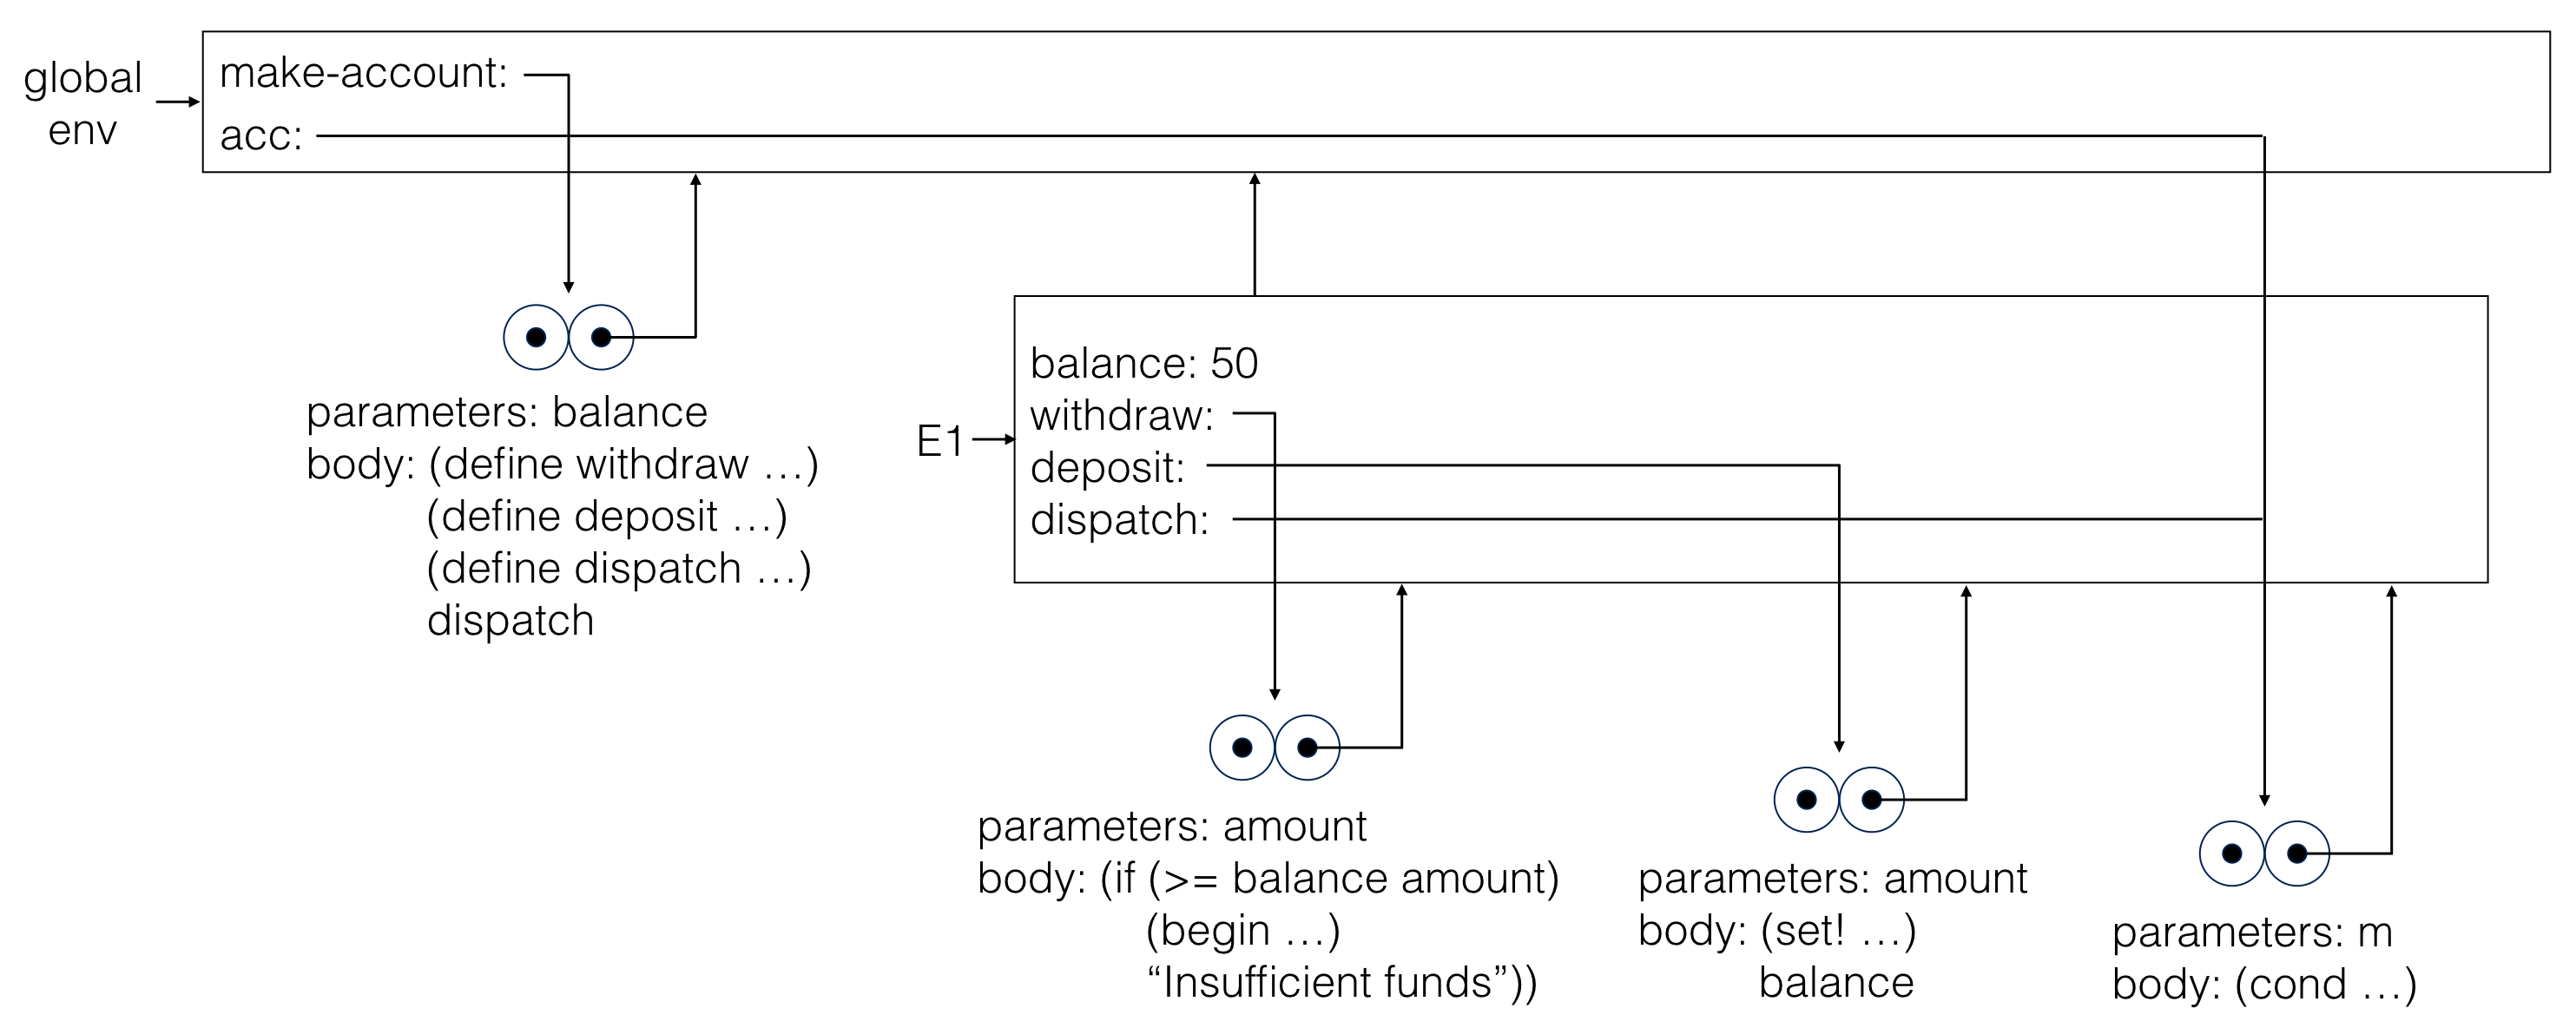
\includegraphics[width=15cm]{ex-3.11-1.png}
\end{center}

The environments created by applying the procedure object (acc 'deposit) to 40 are given as follows:

\begin{center}
    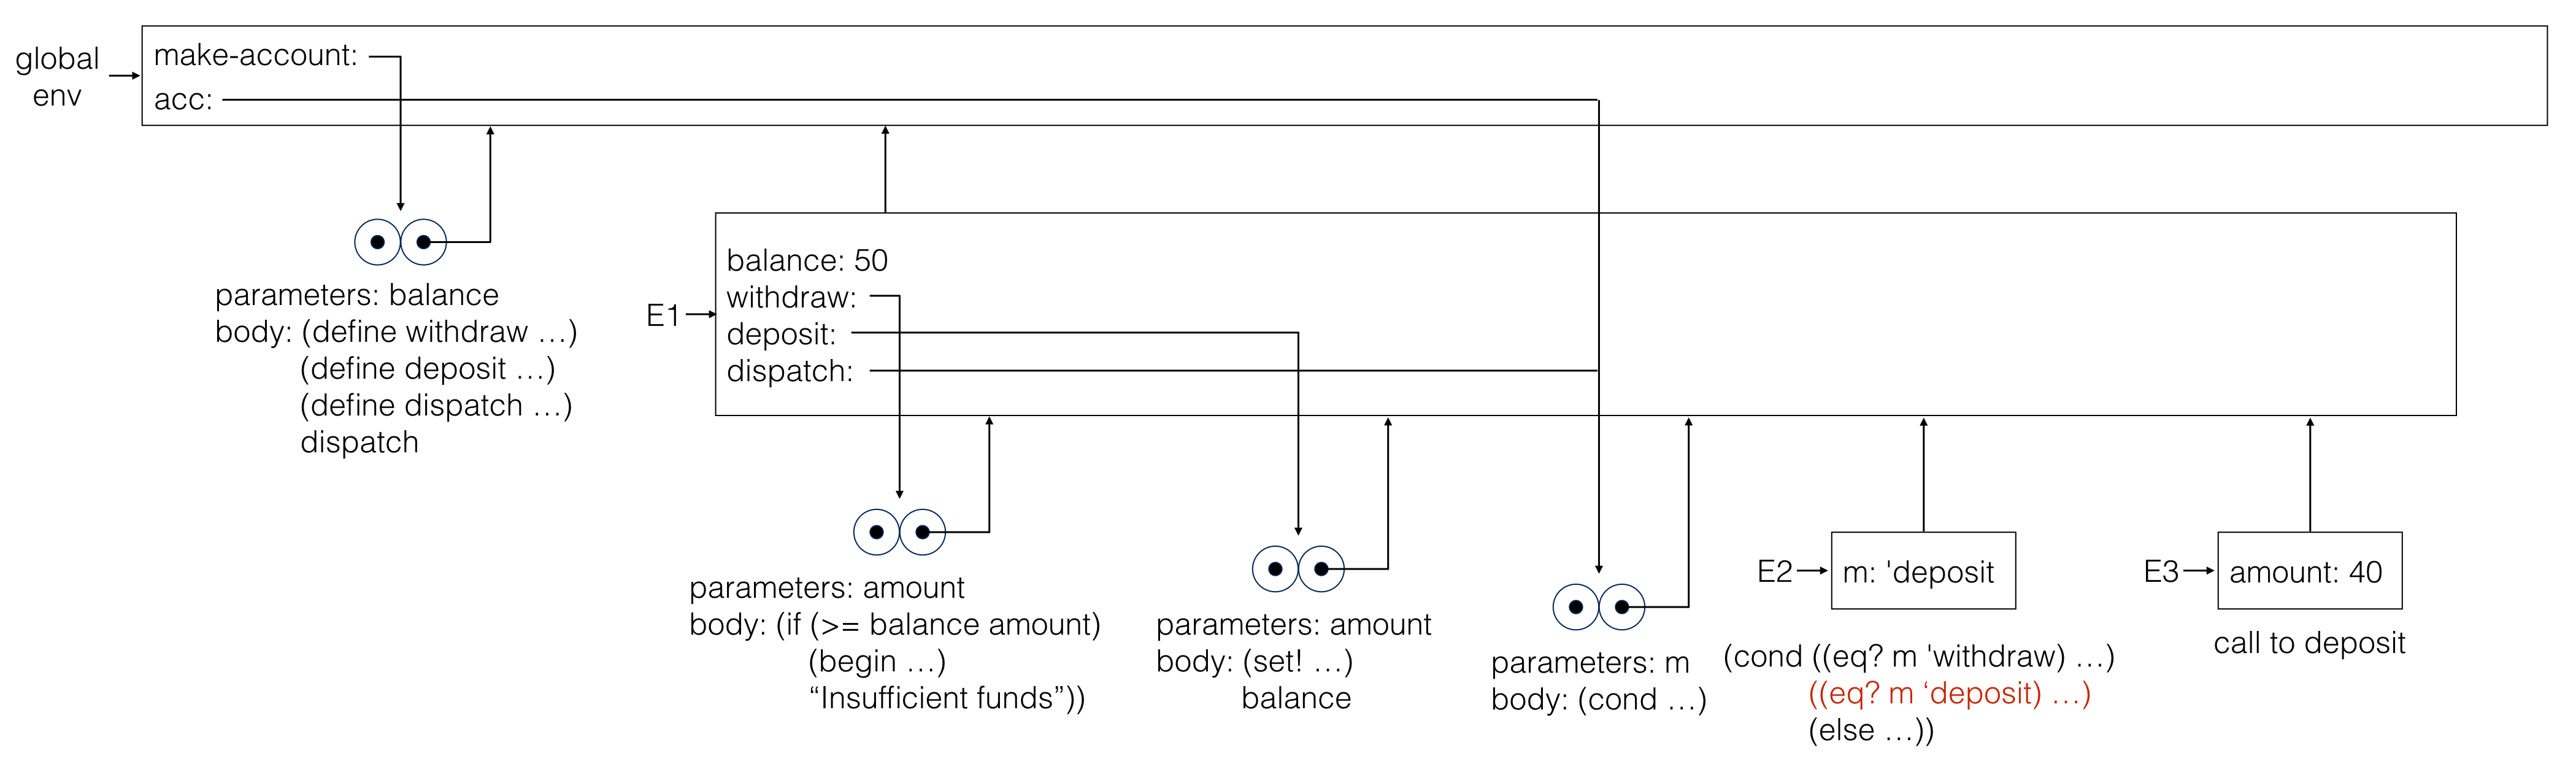
\includegraphics[width=15cm]{ex-3.11-2.png}
\end{center}

After the call to (acc 'deposit), the environments become

\begin{center}
    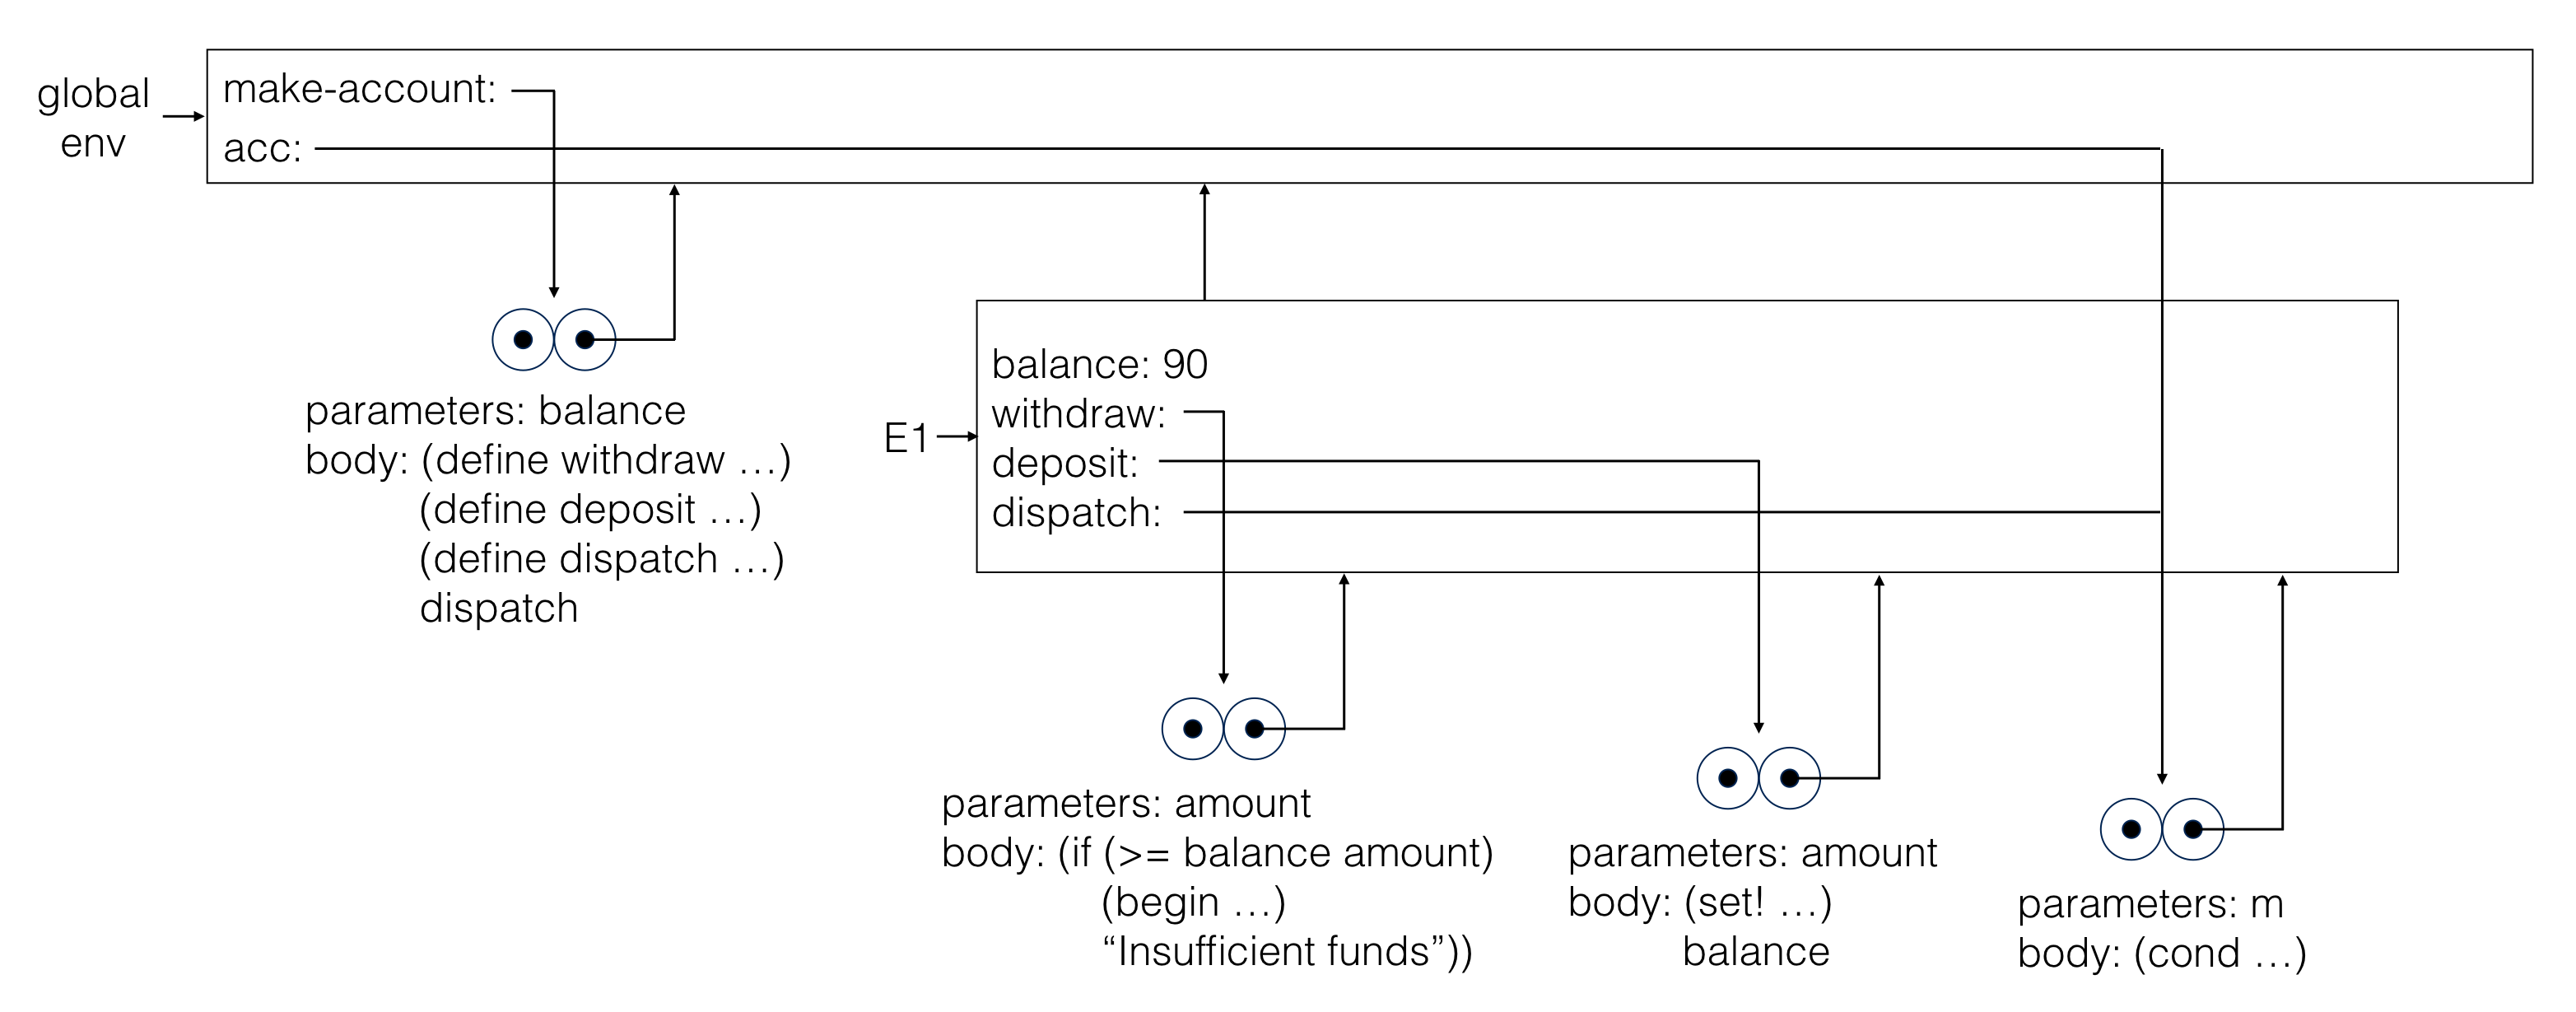
\includegraphics[width=15cm]{ex-3.11-3.png}
\end{center}

The environments created by applying the procedure object (acc 'withdraw) to 60 are given as follows:

\begin{center}
    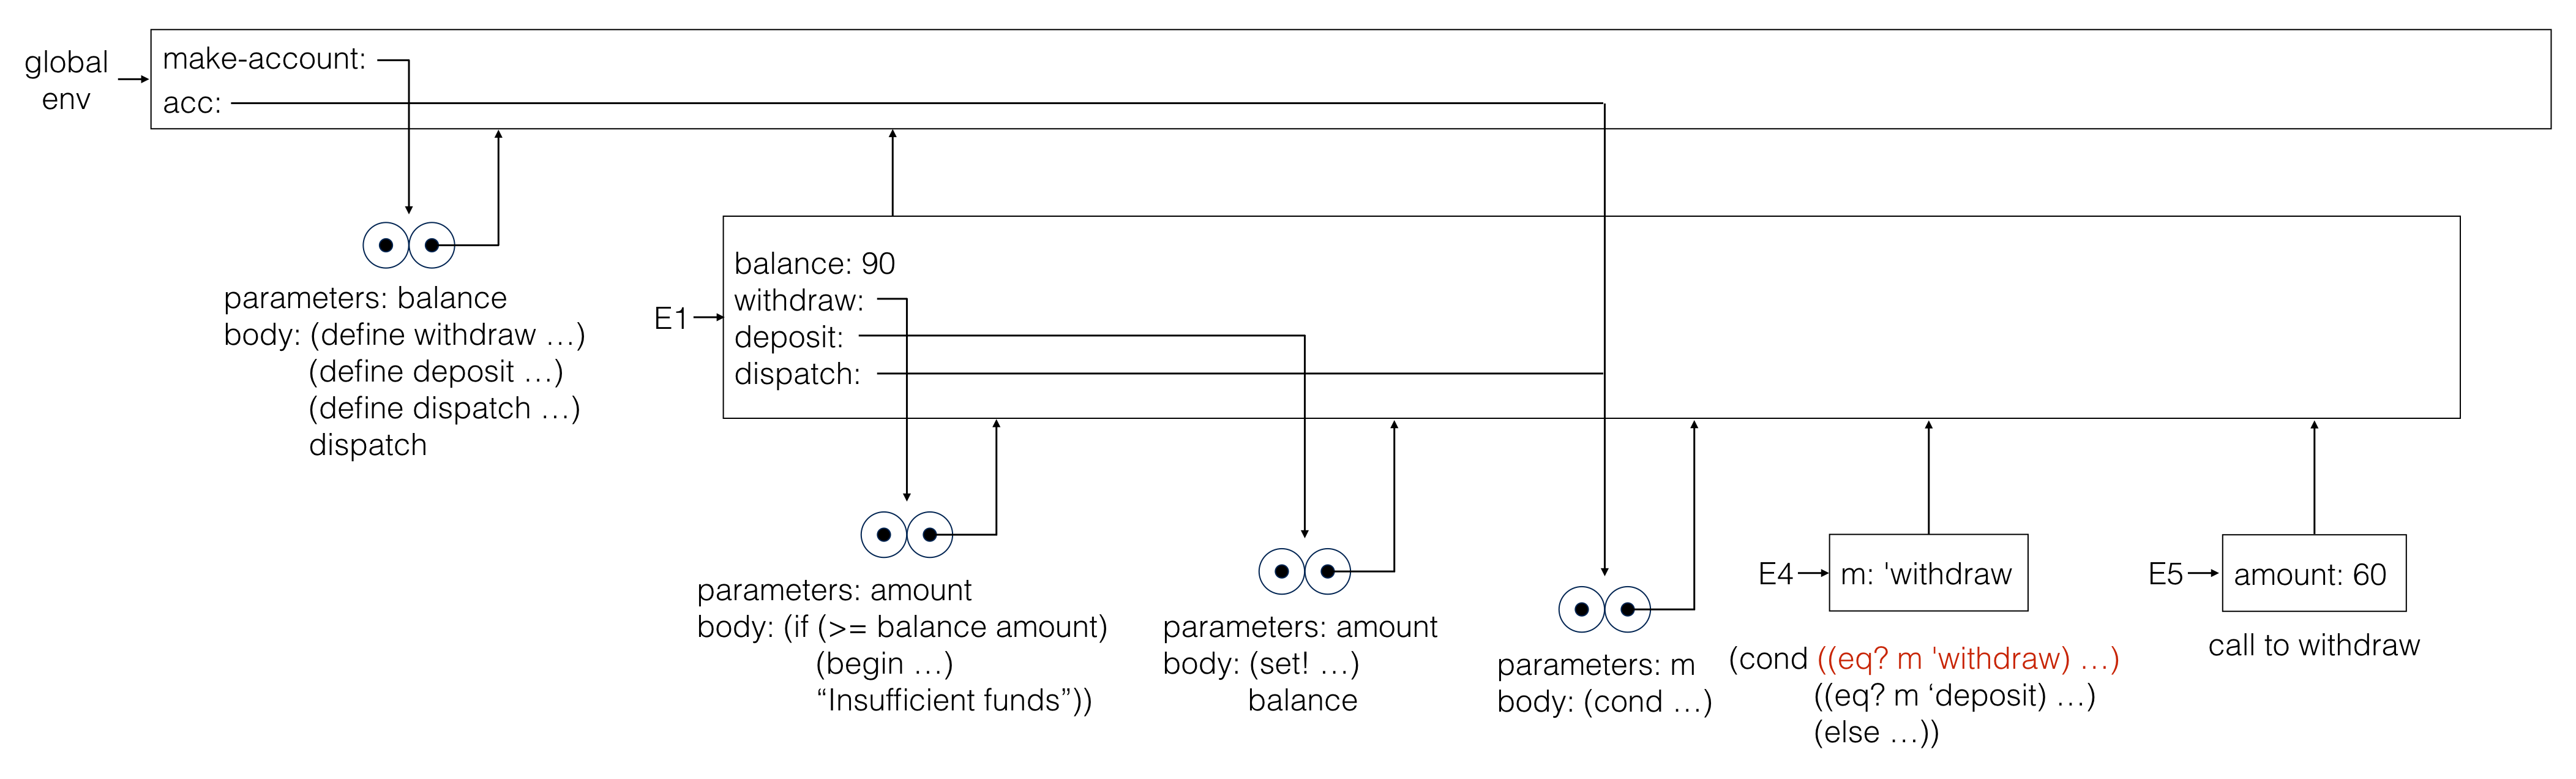
\includegraphics[width=15cm]{ex-3.11-4.png}
\end{center}

After the call to (acc 'withdraw), the environments become

\begin{center}
    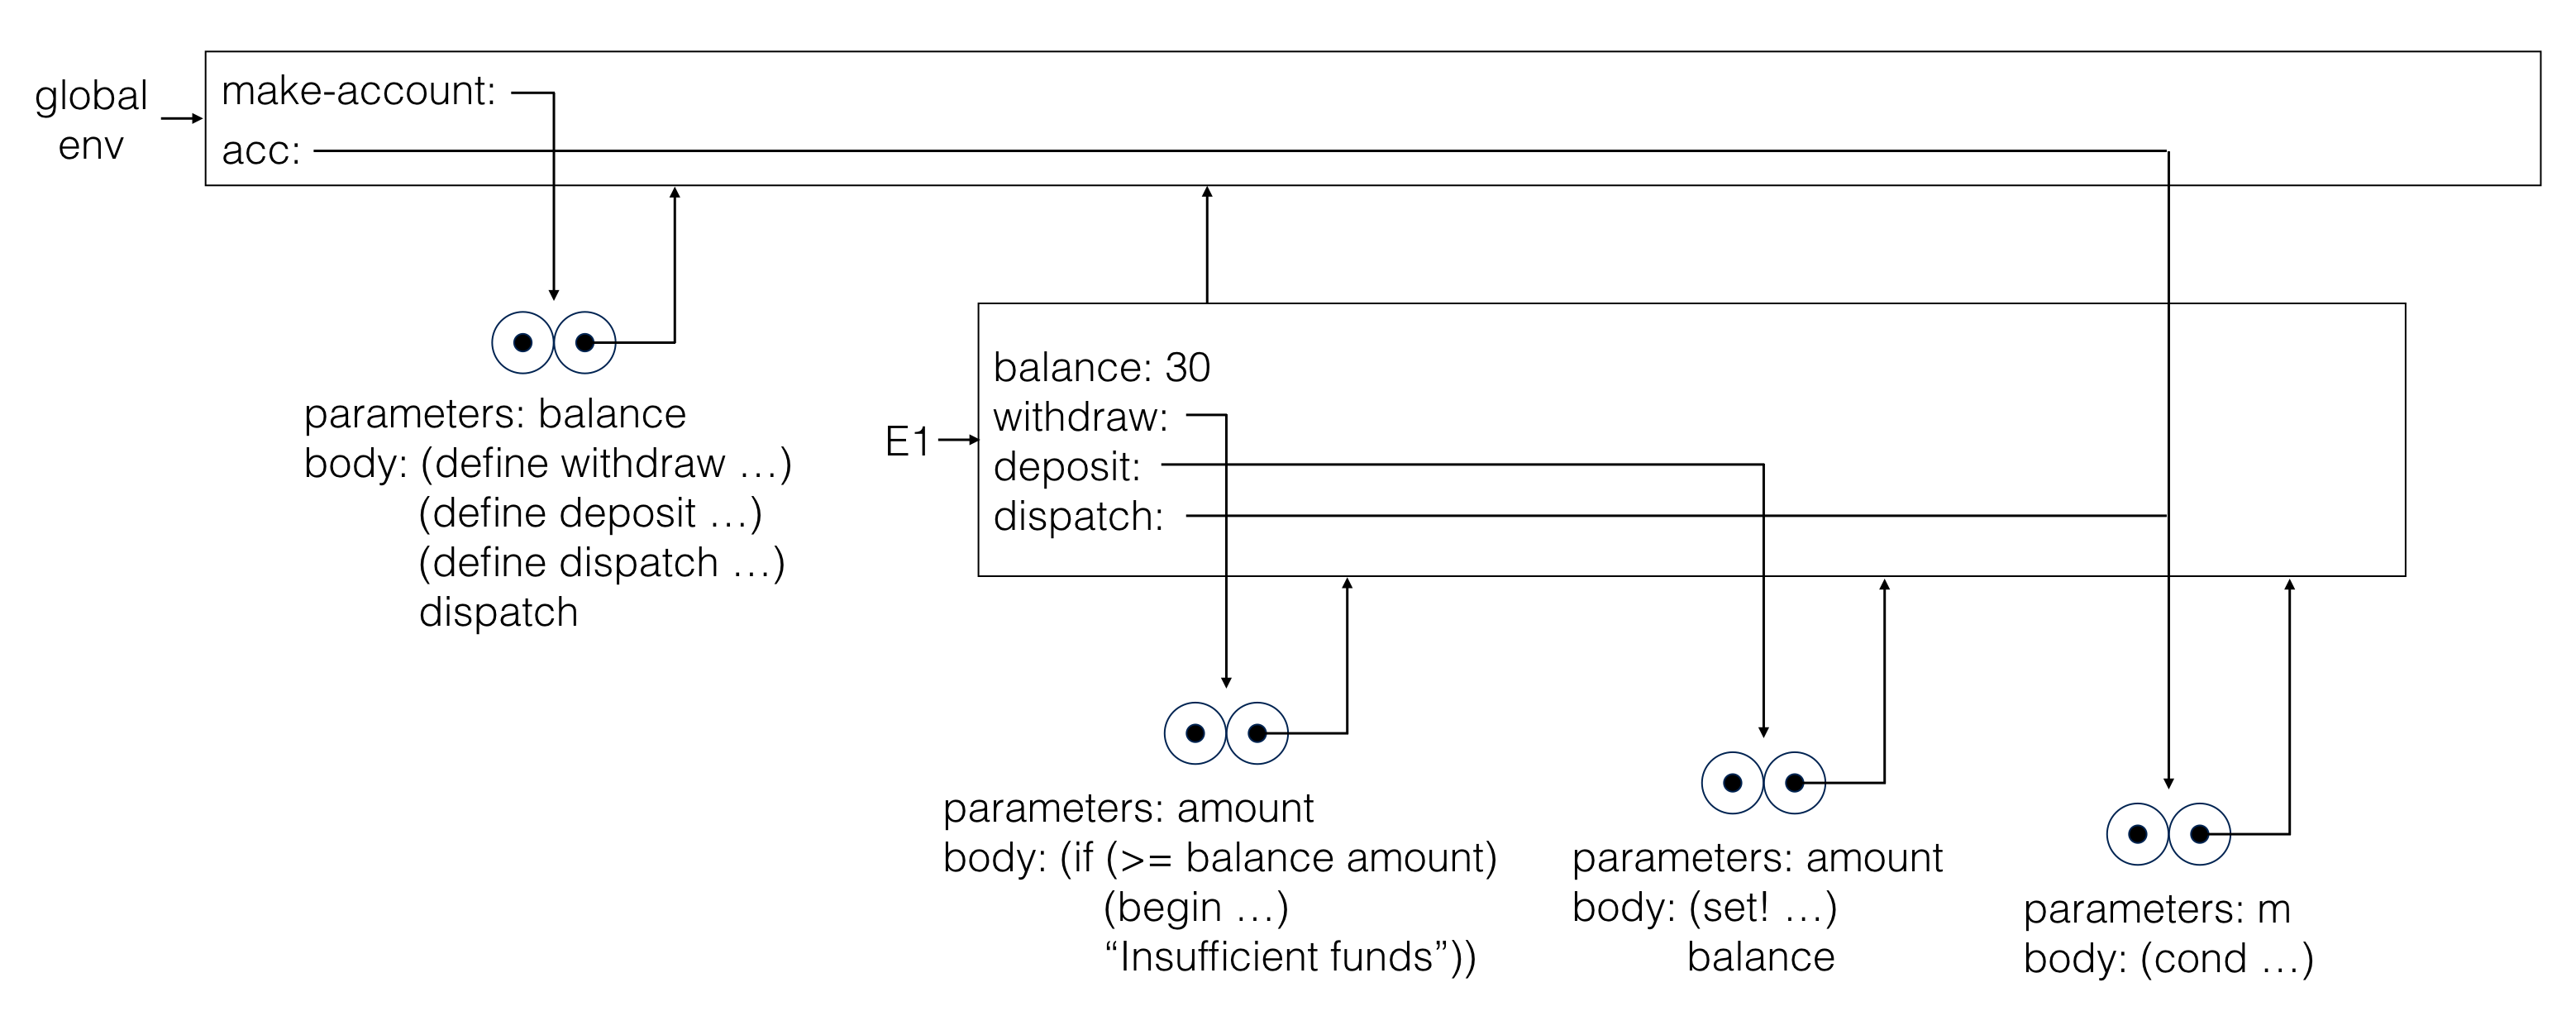
\includegraphics[width=15cm]{ex-3.11-5.png}
\end{center}

The local state for \url{acc}, i.e. the state variable \url{balance} and the three internal procedures \url{withdraw}, \url{deposit} and \url{dispatch}, is kept in the first frame of the environment \url{E1}, whose enclosing environment is the global environment.

After defining another account \url{acc2} as (define acc2 (make-account 100)), the state local state for \url{acc2}, i.e. the state variable \url{balance} and the three internal procedures \url{withdraw}, \url{deposit} and \url{dispatch}, is kept in a separate environment whose enclosing environment is the global environment. Furthermore, the global environment and code for each procedure are shared between \url{acc} and \url{acc2}.

\end{document}
